
%!TEX root = /Users/leicester/data/master/SS08/AS/Ausarbeitung/as-ausarbeitung.tex
%
% HEADER
%

\documentclass[pdf,
12pt, % Schriftgr��e 12?
%	draft, % zur schnelleren Anzeige und zum Auffinden zu voller/leerer Boxen
	oneside, % einseitige Ausgabe
%	abstracton, % Abstract/Zusammenfassung einf�gen
	pdftex, % Ausgabe mit pdftex
	a4paper, % Ausgabe auf A4
	titlepage, % Titelseite ausgeben
	halfparskip, % halbzeiliger Abstand zwischen Abs�tzen
%	idxtotoc, % Index im Inhaltsverzeichnis auff�hren
	bibtotoc % Literaturverzeichnis im Inhaltsverzeichnis auff�hren
	]{scrartcl}
	
\usepackage[utf8]{inputenc}
\usepackage[ngerman]{babel}
\usepackage[T1]{fontenc}

\usepackage{enumerate}

 % defines wrapfigure and wrapfloat
\usepackage{wrapfig}	       


% Paket f�r Graphiken
%\usepackage{graphicx}
\usepackage[dvips]{graphicx}            % to include images

% R�nder einstellen
%\usepackage[left=5cm,right=1.5cm,top=1cm,bottom=2cm,includeheadfoot]{geometry}


% Umgebung f�r Kapitelseiten und Inhatsverzeichnis setzen
\usepackage{fancyhdr} 
\pagestyle{fancy} 
% with this we ensure that the chapter and section 
% headings are in lowercase 
%\renewcommand{\chaptermark}[1]{markboth{#1}{}} 
%\renewcommand{\sectionmark}[1]{\markright{\thesection\ #1}} 
\fancyhf{} %delete the current section for header and footer
\fancyfoot[EC,OC]{\bfseries\thepage} 
\renewcommand{\headrulewidth}{0.5pt}
%\renewcommand{\footrulewidth}{0.5pt}
% make space for the rule 
\fancypagestyle{plain}{% 
\fancyhead{} %get rid of the headers on plain pages 
\renewcommand{\headrulewidth}{0} % and the line 
}





% Paket f�r Farben im PDF laden
\usepackage{color}

% Linkfarbe setzen
%\definecolor{LinkColor}{rgb}{0,0,0.5}
\definecolor{LinkColor}{rgb}{0,0,0}

% Links im PDF aktivieren und PDF-Optionen setzen
\usepackage[%
	pdftitle={},%
	pdfauthor={anonymus},%	
	pdfsubject={},
	pdfkeywords={}]{hyperref}

% Linkfarben setzen
\hypersetup{colorlinks=true,%
	linkcolor=LinkColor,%
	citecolor=LinkColor,%
	filecolor=LinkColor,%
	menucolor=LinkColor,%
	pagecolor=LinkColor,%
	urlcolor=LinkColor}
	
	
%%  Zitieren
\usepackage[
square, %for square brackets;
numbers % for numerical citations;
]{natbib}


%%% Kopfzeile
\subject{Ausarbeitung}
\title{}
%\author{Tim Haussmann\\mim103@gm.fh-koeln.de}


%Hurenkinder und Schusterjungen verhindern
\clubpenalty = 10000
\widowpenalty = 10000 \displaywidowpenalty = 10000




\usepackage{subfig} 






%% EOF
%


\begin{document}
	
	
	% Aussehen der Captions fuer subfigures (subfig-Paket)
	 \captionsetup[subfloat]{%
	   margin = 10pt,
	   font = {small,rm},
	   labelfont = {small,bf},
	   format = plain, % oder 'hang'
	   indention = 0em,  % Einruecken der Beschriftung
	   labelsep = space, %period, space, quad, newline
	   justification = RaggedRight, % justified, centering
	   singlelinecheck = true, % false (true=bei einer Zeile immer zentrieren)
	   position = bottom, %top
	   labelformat = parens % simple, empty % Wie die Bezeichnung gesetzt wird
	 }
	
	
	

%Leeres Vorblatt
\newpage
\thispagestyle{empty} 



%!TEX root = /Users/ede/Documents/Master/19_AS/Ausarbeitung/as-ausarbeitung.tex
%
%
% Titelseite der Arbeit
%
%

\begin{titlepage}
\center
\vspace*{4em}
\large \textbf{\textsc{Advanced Seminar}}\\ 
\vspace{1em}
%\huge\textbf{{\sffamily Extraction von Verkehrsinformationen aus GPS-Logs}}
\huge\textbf{{\sffamily Tag-Rankingverfahren für Bilder}}
\vspace{3em}

\large
\textsc{Dozent}\\
 Prof. Dr. Kristian Fischer \\
\vspace{1em}
 Fachhochschule Köln, Campus Gummersbach\\
\vspace{8em}







% \vspace{8em}
%  \large Tim Haussmann\\
%  \large mim103@gm.fh-koeln.de\\
\vspace{17em}
Köln, \today
\end{titlepage}

\begin{abstract}
Die semantische Beschreibung von Daten im Internet gewinnt immer mehr Bedeutung. Tagging als einfache Variante der Ontologie-freien Beschreibung erfreut sich in vielen Bereichen großer Beliebtheit. Es erlaubt effektiveres Suchen und Einordnen im Vergleich zu bisherigen Suchansätzen. Vor allem bei sozialen Netzwerken wie Flickr entstehen viele Annotationen. Dabei müssen die Tags nach ihrer Relevanz zum Inhalt des Bildes priorisiert werden. Ranking Verfahren beschreiben Möglichkeiten, die ungeordneten Tags mit Relevanzinformationen anzureichern und damit zu bewerten. 
\end{abstract}

%\maketitle
\tableofcontents
\newpage
\listoffigures
\listoftables

%!TEX root = /Users/ede/Documents/Master/19_AS/Ausarbeitung/as-ausarbeitung.tex
\section{Motivation}

Durch erhöhte Bandbreiten und neue Techniken fand in den letzten Jahren eine hohe Zunahme an Multimedia Objekten im Internet statt. Die Multimedia Daten werden dabei sowohl auf privaten Webseiten als auch in sozialen Netzwerken wie Youtube\footnote{http://www.youtube.com}, Facebook\footnote{http://www.facebook.com} und auch das in diesem Paper näher behandelte Flickr\footnote{http://www.flickr.com} verfügbar gemacht.

Menschen suchen in der Regel Stichwort-basiert. Sie geben der Suchmaschine ein oder mehrere Schlüsselwörter, die in irgendeiner Beziehung zu den gesuchten Inhalten stehen. Um nun eine erfolgreiche Suche nach Multimedia Objekten zu ermöglichen, müssen die Medien nach \cite{collectiveKnowledge} reichhaltige Metadaten aufweisen, um eine Beziehung zwischen den Suchparametern und den durch die Suchmaschine indizierten Inhalten herzustellen. 

Die automatische Metadaten-Erstellung kostet nur wenig menschlichen Aufwand, nach \cite{combiningMultipleEvidence} ist es aber bisher nicht ausreichend für den praktischen Einsatz. Im Gegensatz zu reinem Text ist die automatische Extraktion von Metadaten aus Multimedia Objekten jedoch weitaus schwieriger. Die von Maschinen extrahierten Eigenschaften aus Multimedia Objekten sind zur Zeit noch auf einer zu niedrigen semantischen Ebene, so dass kein Bezug zu den Suchwörtern hergestellt werden kann. Der umgebende Text von Multimedia Daten, wie dies in Webseiten üblich ist, kann ebenfalls nur bedingt als Quelle für Metadaten genutzt werden, da dieser falsche oder unzureichende Angaben enthalten kann.

Somit ist die manuelle Generierung von Metadaten genauer und im Moment praktischer als die automatische Annotation. Weiterhin zeigt die rege Nutzung von sozialen Netzwerken, mit ihren Möglichkeiten der manuellen Annotation von Medien, dass diese Arbeit von den Autoren durchaus geleistet wird. Laut \cite{whyWeTag} sind die Gründe für das Taggen meist damit motiviert, dass die Urheber von Medien diese für die gesamte Nutzerschaft besser auffindbar machen wollen. 

Optimal wäre dabei die Verwendung von Ontologien zum Kennzeichnen und Einordnen der Objekte. Dieses Vorgehen ist jedoch nur für spezielle Fachgebiete möglich. Zunächst ist der Aufwand für die Erstellung solcher Ontologien sehr hoch und kostenaufwendig (siehe \cite{ontology_expensive1} und \cite{ontology_expensive2}). Aber auch die Verwendung vorgegebener und vor allem oft unbekannter Strukturen fällt den meisten Benutzern im Internet sehr schwer und erfordert relativ aufwendige Einarbeitung.

Eine vereinfachte Version der Generierung von Metadaten für Medienobjekte ist das \emph{Tagging} beziehungsweise \emph{Social Tagging}. Dabei geben die Nutzer einem Objekt frei gewählte Schlagwörter. Hierbei wird keine Taxonomie oder Ontologie vorgegeben und die Annotation wird aufgrund der einfachen Verfahrensweise von einer großen Anzahl von Menschen durchgeführt. Diese Art von Organisation wird auch \emph{Folksonomy} genannt.

Dabei gibt es eine Reihe von Problemen, die den Vorgang des Taggings erschweren beziehungsweise schlechte Ergebnisse liefern. Falsche, irrelevante und fehlende Tags führen jedoch zu schlechten Suchergebnissen.

\begin{itemize}
  \item \textbf{Synonyme:} Laut \cite{learningToTag} vergeben Menschen unterschiedliche Tags für die gleichen Objekte. Dies rührt daher, dass Menschen unterschiedliche Begriffe für die gleichen Objekte verwenden. Es ist gleichzeitig auch schwierig für den Benutzer alle zu einem Objekt passenden Begriffe zu finden.
  \item \textbf{Mehrdeutigkeit:} Benutzer verwenden allgemeine, mehrdeutige Begriffe, die ein Objekt nicht eindeutig beschreiben. Zum Beispiel könnte der Tag \emph{apple} die Annotation für eine Marke oder eine Frucht sein. Dabei wissen die Nutzer oft nicht mal etwas von der anderen Bedeutung oder erinnern sich nicht an die mit dem Objekt assoziieren Begriffe.
  \item \textbf{Semantischer Verlust:} Nicht alle Gegenstände und Informationen die in dem Medienobjekt enthalten sind werden annotiert.
  \item \textbf{Semantisches Rauschen:} Teilweise enthalten Medienobjekte Annotationen die keinen Zusammenhang zu dem Objekt besitzen.
\end{itemize}


Eine genaue Analyse und Klassifizierung der in Folksonomies enthaltenen Tags erfolgt in dem Kapitel \ref{sec:analyse_und_klassifikation}.

\subsection{Tag Ranking} % (fold)
\label{sub:tag_ranking}

% - mögliche Lösungen/Ansätze um Probleme zu reduzieren/beseitigen:
Um einige der oben genannten Probleme zu beseitigen oder wenigstens ihre Auswirkungen zu reduzieren, werden die Tags hinsichtlich ihrer Relevanz für das Medienobjekt untersucht und priorisiert. Es wird also ein Ranking, zu deutsch Einordnung oder Bewertung vorgenommen. Diese Ausarbeitung geht auf zwei solcher Tag-Ranking Algorithmen ein. Dabei werden unterschiedliche Ansätze gewählt, die sich hinsichtlich ihrer Herangehensweise und den Ergebnissen unterscheiden. Die den Verfahren vorangestellten Analysen werden in Kapitel \ref{sec:analyse_und_klassifikation} beschrieben, anschließend die Verfahren in Kapitel \ref{sec:tag_ranking_verfahren} im genauen vorgestellt und die Ergebnisse in Bezug auf Qualität und Performanz verglichen und bewertet.

\begin{figure}[htbp]
  \centering
    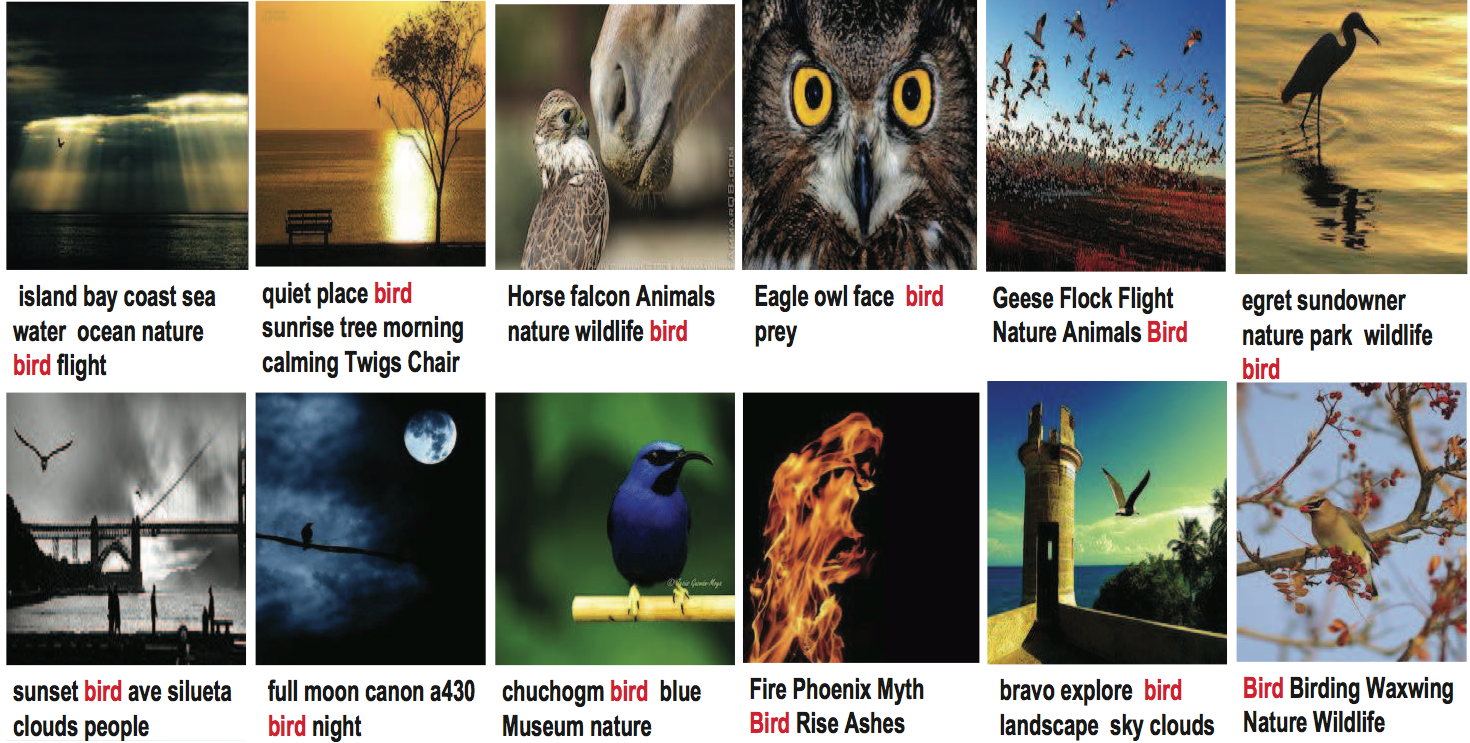
\includegraphics[height=0.5\textwidth]{images/bird_search_results_wide.png}
  \caption{Suchergebnisse bei einer Tag-basierten Flickr Suche nach \emph{bird} aus \cite{ranking}. Aus Platzgründen wird nur eine Auswahl von Tags pro Photo angegeben.}
  \label{fig:images_bird_search_results}
\end{figure}

Die aus der Anwendung der Algorithmen resultierende Vorteile liegen in besseren Suchergebnissen bei einer Stichwort basierten Suche und einem stark vereinfachten Tagging Prozess für den Benutzer sowie allgemein gesteigerter Relevanz der Tags. Abbildung \ref{fig:images_bird_search_results} veranschaulicht die Nachfrage für diese Art von Algorithmen. Zu sehen sind mehrere Bilder mit den annotierten Tags, die als Suchergebnis für das Suchwort \emph{bird} von Flickr ausgegeben werden. Man erkennt zunächst, dass die Tags nicht nach Relevanz für das jeweilige Bild sortiert sind und einige der Photos nicht zur Anfrage passen.


% subsection tag_ranking (end)

\subsection{Anwendungsgebiete von Tags} % (fold)
\label{sub:anwendungsgebiete}

Wie oben schon erwähnt, werden Tags für die Suche nach Medienobjekten verwendet. Hierfür ist es besonders wichtig, dass die Tags Relevanzinformationen zu den assoziierten Medienobjekten aufweisen, um die Ergebnisse für den Benutzer in einer priorisierten Reihenfolge in Bezug zu der Suchanfrage auszugeben. Die ist vergleichbar mit den Suchergebnissen bei Google, die nach ihrer relativen Relevanz zu dem Suchbegriff und der objektiven Wichtigkeit der präsentierten Inhalte sortiert werden (siehe hierzu \cite{googlePageRank}).

Das zweite, wichtige Einsatzgebiet von Tags ist das Vorschlagen von Tags beim Tagging Prozess. Hierbei werden die gleichen Relevanzinformationen verwendet, um dem Benutzer die Annotations-Aufgabe zu erleichtern und dabei die Ergebnisse zu verbessern. Dabei werden auf Basis der bereits eingegebenen Tags weitere, damit assoziierte und relevante Tags vorgeschlagen, so dass der Benutzer diese nur noch auszuwählen braucht.

Diese Ausarbeitung beschäftigt sich vor allem mit dem zweiten Anwendungsfall und geht in den folgenden Kapiteln näher auf die Verfahren ein.

%  TODO: rein oder raus:
 % - Vorschlagen von Gruppen für Photos

% subsection anwendungsgebiete (end)


% Fischer: Mir wäre dabei wichtig, dass Sie einen klaren Schwerpunkt setzen und ausgewählte Verfahren in die Tiefe behandeln.
% 
% Aufbau: 
%  - Kurze Einführung in das Gebiet des Taggings und Problembeschreibung
%  - Anwendungsgebiete der Ranking-Verfahren als Motivation
%  - Vorstellung der Ansätze um Bilder-Tags zu werten
%  -

%!TEX root = /Users/ede/Documents/Master/19_AS/Ausarbeitung/as-ausarbeitung.tex
\section{Analyse und Klassifikation} % (fold)
\label{sec:analyse_und_klassifikation}

Um die Tag-Rankingverfahren hinsichtlich der oben genannten Anwendungsgebiete zu formulieren und zu optimieren, müssen zunächst die vorhandenen Tags in einer Folksonomy analysiert werden \cite{collectiveKnowledge}. Als Datenbasis aller vorgestellten Ansätze dient die Photocommunity Flickr. Diese Photocommunity Plattform beinhaltet das Konzepts des Tagging und verfügt über eine hohe Anzahl\footnote{Am 12.10.09 erreichte der Bestand von Flickr.com über 4 Milliarden Photos, vgl. http://blog.Flickr.net/en/2009/10/12/4000000000/ } von frei verfügbaren Photos


%TODO: mehr beschreiben, wofür die Analyse und Klassifikation benötigt wird, und was als Ergbenis erwartet wird(z.B. Dass folgende Fragen beantwortet werden)
Damit die Anwendungsgebiete möglichst unterstützen werden können, ist ein genaues Verständnis der Vorgehensweise beim Tagging wichtig. Ebenso ist die Motivation hinter dem Tagging von Bedeutung, also warum Menschen ihre Daten überhaupt annotieren und welches Ziel sie damit verfolgen. Dazu werden mehrere Untersuchungen über eine große Menge von Photos aus Flickr vorgestellt.

Im Folgenden soll kurz auf die Analyse der Tags eingegangen werden, wobei die nachstehenden Fragen beantwortet werden sollen:
\begin{itemize}
	\item     Welche Tags sind vorhanden? Frequenz der Tags?
	\item     Wie gehen Benutzer beim Taggen vor?
	\item     Warum taggen Benutzer?
	\item     In welcher Reihenfolge liegen die Tags vor?
  \item     Anzahl der Tags pro Photo?
	\item     In welchen Beziehungen stehen die Tags untereinander?
	\item     In wie weit gleicht der Inhalt der Photos, wenn gleiche Tags vorhanden sind?
	\item     Können die Tags in Kategorien zusammengefasst werden?
\end{itemize}

Die nächsten Abschnitte beschreiben also zunächst die in Flickr vorhandenen Photos sowie die zugehörigen Tags und klassifizieren diese anschließend, um sie für die Tag Ranking Verfahren sowie für die Evaluation der Verfahren nützlich zu machen.

\subsection{Analyse der Tags und Photos} % (fold)
\label{sub:analyse_der_tags}

\cite{collectiveKnowledge} verwenden über 52 Millionen Photos aus den Jahren 2004 bis 2007 für ihre Untersuchung. Die vorgenommene Auswahl verfügt über 188 Millionen Tags, wovon 3,7 Millionen eindeutig sind. Dies ist also eine statistisch ausreichende Menge, um auf die Gesamtheit schließen zu können.

\begin{figure}[htbp]
    \centering
      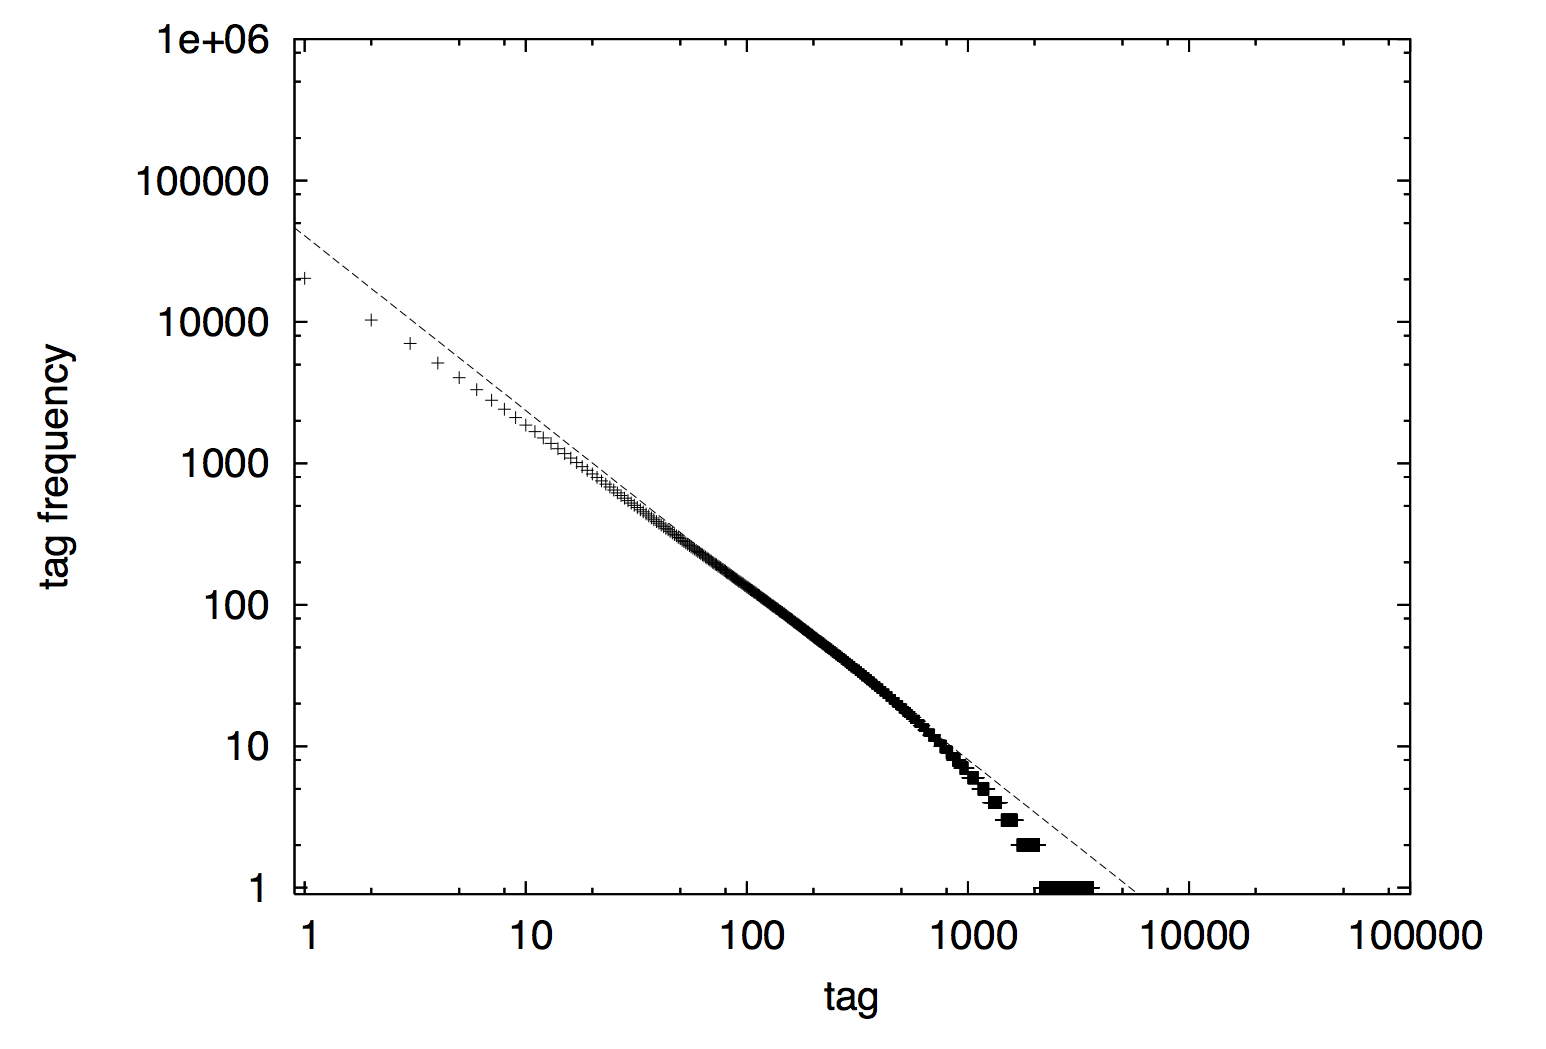
\includegraphics[height=2in]{images/collectiveKnowledge_tag_frequency.png}
    \caption{Häufigkeitsverteilung von 3,7 Millionen eindeutigen Tags in Flickr aus \cite{collectiveKnowledge}. Die Achsen sind hierbei logarithmisch skaliert.}
    \label{fig:images_collectiveKnowledge_word_net_categories}
\end{figure}

Abbildung \ref{fig:images_collectiveKnowledge_word_net_categories} veranschaulicht die Häufigkeitsverteilung der Tags. Die Abszisse repräsentiert die 3,7 Millionen eindeutigen Tags sortiert nach absteigender Häufigkeit, während die Ordinate die Häufigkeit selbst darstellt. Die ablesbare Kurve wird sehr gut durch das Potenzgesetz  beschrieben, vgl. \cite{hpParetoPowerLaw}. Dieses besagt für beobachtete Phänomene in der Welt, dass geringe Vorkommnisse sehr häufig und große Anhäufungen sehr selten auftreten. Im vorliegenden Fall werden einige wenige Tags sehr oft von den Benutzer für Annotationen verwendet, wohingegen die meisten Tags nur selten eingesetzt werden.

In Anbetracht der Aufgabe, dem Benutzer passende Tags für die Annotation vorzuschlagen, ist es laut \cite{collectiveKnowledge} nicht sinnvoll die häufigsten Tags anzubieten, da diese zu allgemein in ihrer Bedeutung sind. So sind die fünf am meisten verwendeten Tags \emph{2006, 2005, wedding, party} und \emph{2004}. Analog dazu sind die extrem selten verwendeten Tags zu spezifisch und eigenen sich ebenfalls nur bedingt für die vorgesehene Aufgabe. Diese Verwendungshäufigkeit von Tags fließt in das Verfahren zum Vorschlagen von Tags nach \cite{collectiveKnowledge} ein und wird in Kapitel \ref{sec:tag_ranking_verfahren} erläutert.

Zu einem ähnlichen Ergebnis gelangen auch \cite{learningToTag} in ihrer Untersuchung von über 640 Millionen Photos aus Flickr, welche in Abbildung \ref{fig:images_learning_to_tag_frequency} veranschaulicht wird. Diese Sammlung enthält insgesamt 1,3 Milliarden Tags, wobei die Autoren eine Unterteilung bezüglich der Art der Tags vornehmen. Ein Prozent der Tags werden mehr als 20.000 Mal verwendet, womit diese laut den Autoren nur wenig Information enthalten. Knapp 6\% der Tags werden als populär angesehen, da sie mehr als 5000 Mal in der Sammlung auftauchen. 33,21 Prozent treten zwischen 50 und 5.000 Mal auf und werden zu den spezifischen Tags gezählt. Alle weiteren, seltener auftretenden Tags, die ca. 60 Prozent der Gesamtmenge ausmachen, gelten als Rauschen, das sie meist falsch geschrieben oder einfach nur irreführend sind.

\begin{figure}[htbp]
    \centering
      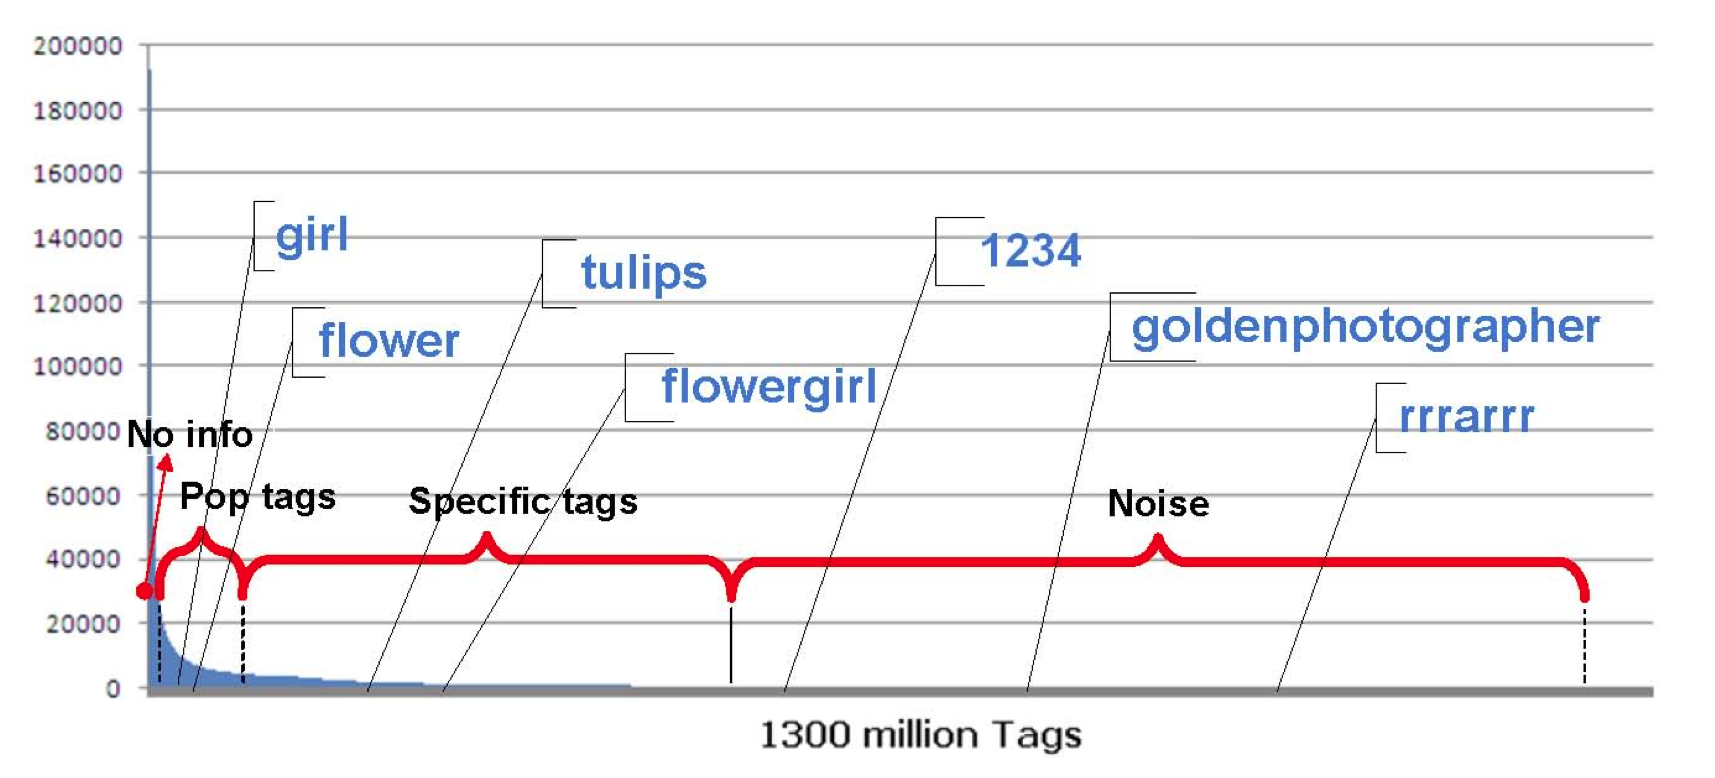
\includegraphics[height=2in]{images/learning_to_tag_frequency.png}
    \caption{Tag Verteilung von über 640 Million Photos aus der Analyse von \cite{learningToTag}, die insgesamt 1,3 Milliarden Tags enthalten.}
    \label{fig:images_learning_to_tag_frequency}
\end{figure}


Bei der Betrachtung der Anzahl der Tags pro Photo zeigt sich ebenfalls eine Verteilung nach dem Potenzgesetz. Laut der Analyse von \cite{collectiveKnowledge} besitzen einige Photos mehr als 50 Tags, der Großteil der Photos mit 64 Prozent Anteil weisen jedoch nur 1 bis 3 Tags auf. Diese Menge eignet sich damit besonders für das Vorschlagen von Tags und zeigt gleichzeitig das Bedürfnis für solche Verfahren.

Jedes Photos in Flickr kann beliebig viele Tags enthalten, wobei diese in der Reihenfolge vorliegen in der sie auch zu dem Photo hinzugefügt wurden. Die Reihenfolge der vergebenen Tags steht dabei in keiner Beziehung zu der Relevanz für das assoziierte Photo. \cite{ranking} untersuchten dazu 1.200 zufällig ausgewählte Photos mit mindestens 10 Tags pro Photo und ließen die Relevanz der Tags für das jeweilige Photo von fünf Probanden bewerten. Nur ein Zehntel der Photos hatte den relevantesten Tag an erster Stelle. Abbildung \ref{fig:images_tag_ranking_psotion_relevant_tag} zeigt die Ergebnisse des Tests mit den Probanden.

\begin{figure}[htbp]
  \centering
    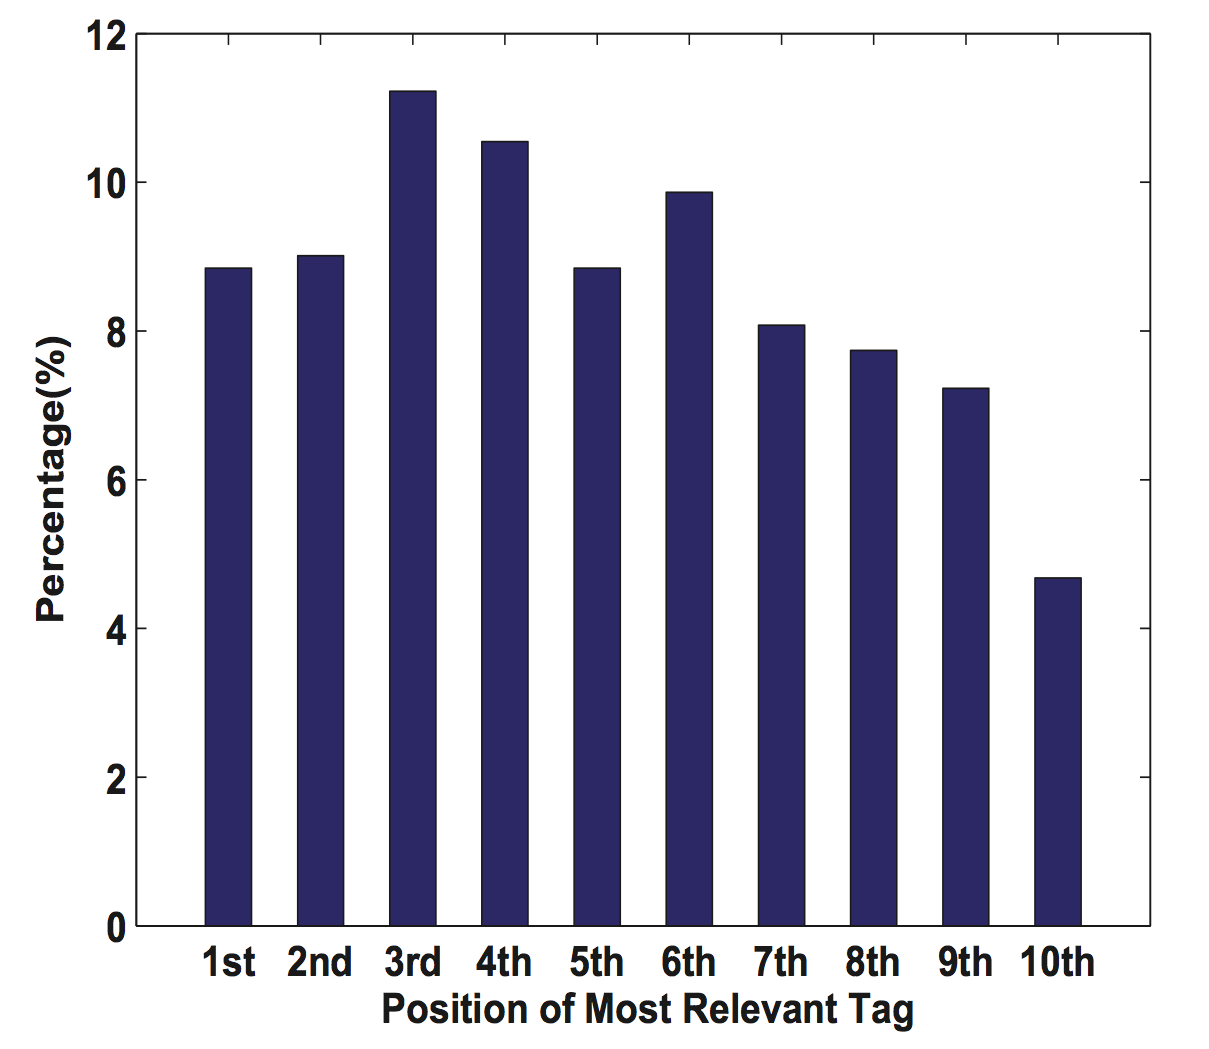
\includegraphics[height=2in]{images/tag_ranking_psotion_relevant_tag.png}
  \caption{Prozentuale Anteile der Photos, die den relevantesten Tag an der n-ten Position der Tag Liste haben. Aus \cite{ranking}}
  \label{fig:images_tag_ranking_psotion_relevant_tag}
\end{figure}
  
Es ist also nicht möglich die Relevanz aus der von Flickr gegebenen Position zu bestimmen. Auffällig ist, dass 70 Prozent aller Photos den relevantesten Tag innerhalb der ersten 10 Positionen haben. Es scheint also ein Zusammenhang zwischen der Eingabesequenz der Tags für ein Photo und der Relevanz des Tags für das Photo zu bestehen, wobei dieser relativ schwach ausgeprägt ist und nicht als qualitative Informationsquelle dienen kann. 

% subsection analyse_der_tags (end)

\subsection{Klassifikation von Tags und Photos} % (fold)
\label{sub:klassifikation_von_tags}

\cite{collectiveKnowledge} untersuchten 52 Millionen Photos und deren Tags aus Flickr. Für die Photos wurde eine Klassifizierung nach der Anzahl gesetzter Tags gewählt. Diese Klassen finden später noch in der Evaluation der Leistung des verwendeten Verfahrens Einsatz. Die Autoren unterteilen die Photos in mehrere Klassen, um das Verhalten des Tag Ranking Verfahrens für Photos mit unterschiedlichem Informationsgehalt der Tags zu analysieren.

\begin{table}[htbp]
\centering
\begin{tabular}{|c|c|c|} 
\hline
 & Tags pro Photo & Anzahl der Photos pro Klasse\\
\hline
Klasse I & 1 & ca. 15,5 Millionen\\
\hline
Klasse II & 2 - 3 & ca. 17,5 Millionen\\
\hline
Klasse III & 4 - 6 & ca. 12 Millionen\\
\hline
Klasse IV & > 6 & ca. 7 Millionen\\
\hline
\end{tabular}
\caption{Definition der Photo-Tag Klassen und die Anzahl der Photos pro Klasse aus \cite{collectiveKnowledge}}
\label{tab:classes_for_tags_collective}
\end{table}





\subsubsection*{Tags} % (fold)
\label{ssub:tags}


Um besser zu verstehen welche Art von Tags die Benutzer vergeben und welche Motive sie taggen, wird in \cite{collectiveKnowledge} eine Abbildung auf die Kategorien aus WordNet\footnote{``Das WordNet ist ein seit 1985 am Cognitive Science Laboratory der Princeton University entwickelter Wortschatz der englischen Sprache.'' aus Wikipedia, abgerufen am 13.12.09.} vorgenommen. Das Ergebnis ist in Abbildung \ref{fig:collectiveKnowledge_word_net_categories} dargestellt.

\begin{figure}[htbp]
  \centering
    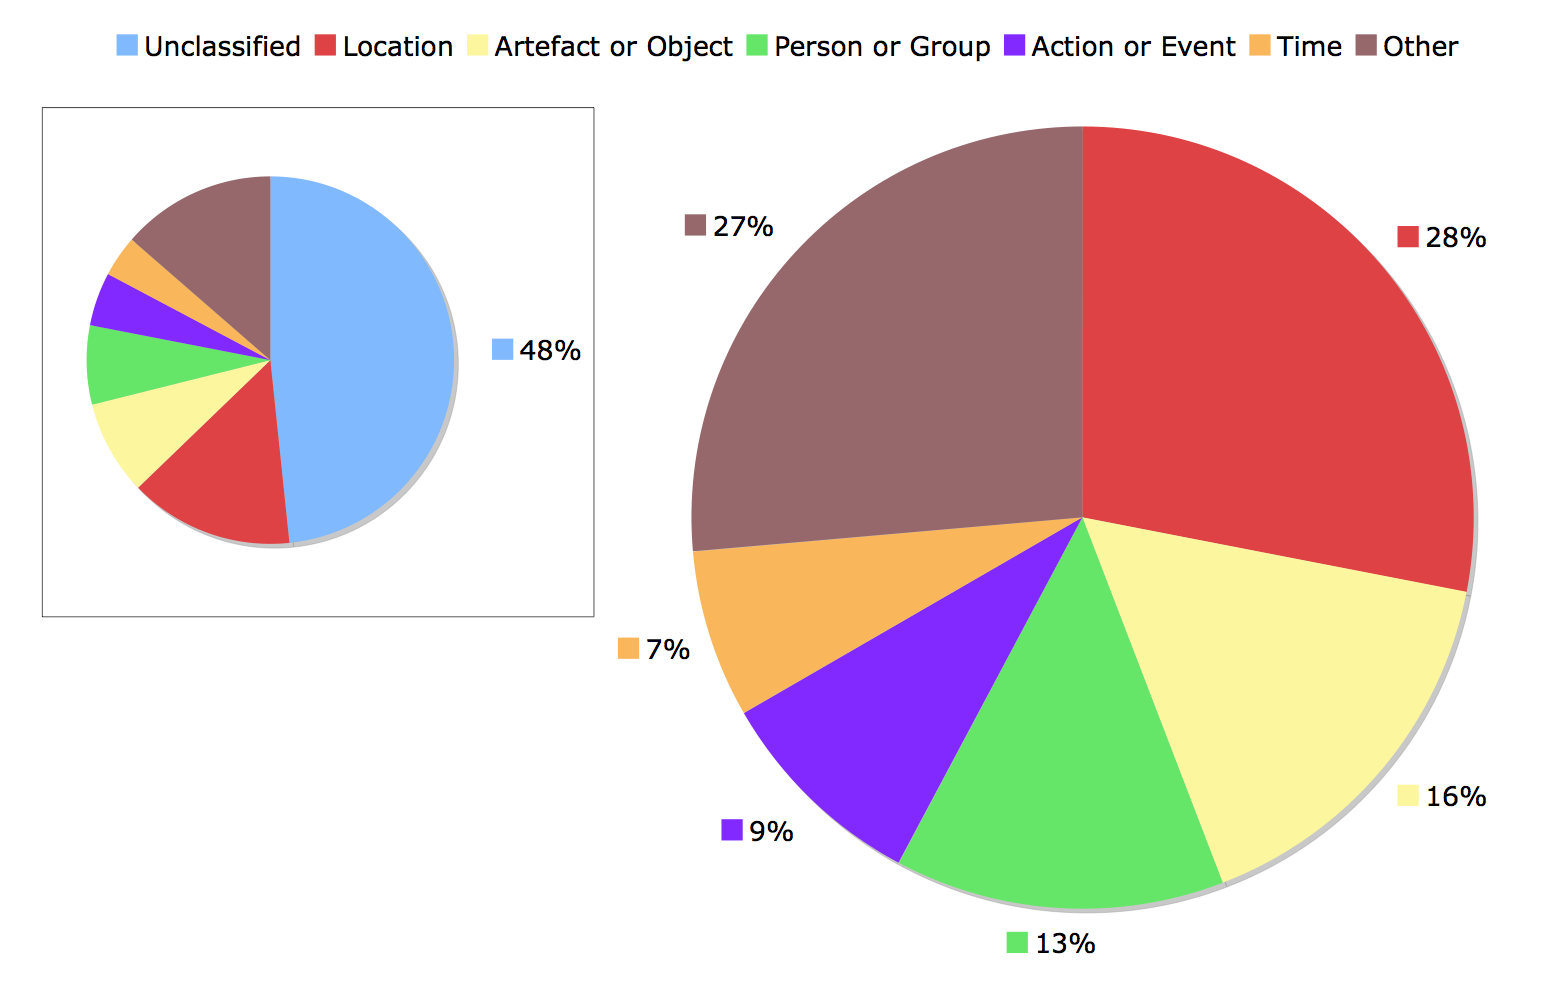
\includegraphics[height=2.5in]{images/collectiveKnowledge_word_net_categories.png}
  \caption{Die häufigsten Kategorien aus WordNet für Flickr Tags nach \cite{collectiveKnowledge}. Das kleine Diagramm zeigt die gesamte Verteilung der WordNet Ergebnisse inklusive der nicht klassifizierten Tags.}
  \label{fig:collectiveKnowledge_word_net_categories}
\end{figure}

52 Prozent der Tags konnten zu WordNet Kategorien zugeordnet werden, die restlichen Tags sind nicht klassifizierbar, das heißt die Begriffe sind nicht im WordNet Katalog enthalten. Dabei wurde, falls mehrere Kategorien für ein Tag in Frage kamen, die als wichtiger eingestufte Kategorie für die Auswertung gewählt. Mit 28 Prozent der klassifizierten Tags erreichen \emph{Ortsangaben} den höchsten Anteil. Weitere Kategorien sind \emph{Menschen oder Gruppen}, \emph{Handlungen oder Ereignisse} und \emph{Zeit}. \cite{collectiveKnowledge} schließen daraus, dass Benutzer nicht nur visuellen Inhalt von Photos, sondern auch Kontextinformationen wie Ort, Zeit und Ereignis annotieren.

Auf Basis dieser Analyse und Klassifikation wurde das Verfahren entwickelt, welches in Abschnitt \ref{sub:ranking_basierend_auf_kollektivem_wissen_nach_zwol} beschrieben wird.

% TODO: Hier noch was mehr zu dem anderen verfahren oder mal was abschließendes und zusammenfassendes

% subsubsection tags (end)  

% subsection klassifikation_von_tags (end)




% section analyse_und_klassifikation (end)

%!TEX root = /Users/ede/Documents/Master/19_AS/Ausarbeitung/as-ausarbeitung.tex
\section{Tag-Ranking Verfahren} % (fold)
\label{sec:tag_ranking_verfahren}
Hier erfolgt die Darstellung der Tag-Ranking Verfahren im genauen.

% 
% 
% \begin{itemize}
%   \item   Visual diversification of image search results \cite{diversification}
%   \item   Tag ranking \cite{ranking}
%   \item   Learning to tag \cite{learningToTag}
%   \item   Learning tag relevance by neighbor voting for social image retrieval \cite{learningtagrelevance}
%   \item   Improving recommendation lists through topic diversification \cite{improvingRecommendations}
%   \item   Why we tag: motivations for annotation in mobile and online media \cite{whyWeTag}
%   \item   Flickr tag recommendation based on collective knowledge \cite{collectiveKnowledge}
% \end{itemize}

\subsection{Ranking basierend auf kollektivem Wissen nach Sigurbjörnsson und van Zwol} % (fold)
\label{sub:ranking_basierend_auf_kollektivem_wissen_nach_zwol_et_al_}

\begin{itemize}
  \item Tag co-occurrence is the key to our tag recommendation approach, and only works reliable when a large quantity of supporting data is available.
  \item We define the co-occurrence between two tags to be the number of photos [in our collection] where both tags are used in the same annotation.
  \item Symmetric measures vs. Asymmetric measures
  \item Zweiter Schritt: Tag Aggregation and Promotion
  \begin{itemize}
    \item Aggregation durch \emph{Vote} und \emph{Sum} Verfahren
    \item Priorisierung der Tags durch \emph{Stability-promotion} und \emph{Descriptiveness-promotion}
  \end{itemize}
\end{itemize}

\begin{figure}[htbp]
  \centering
    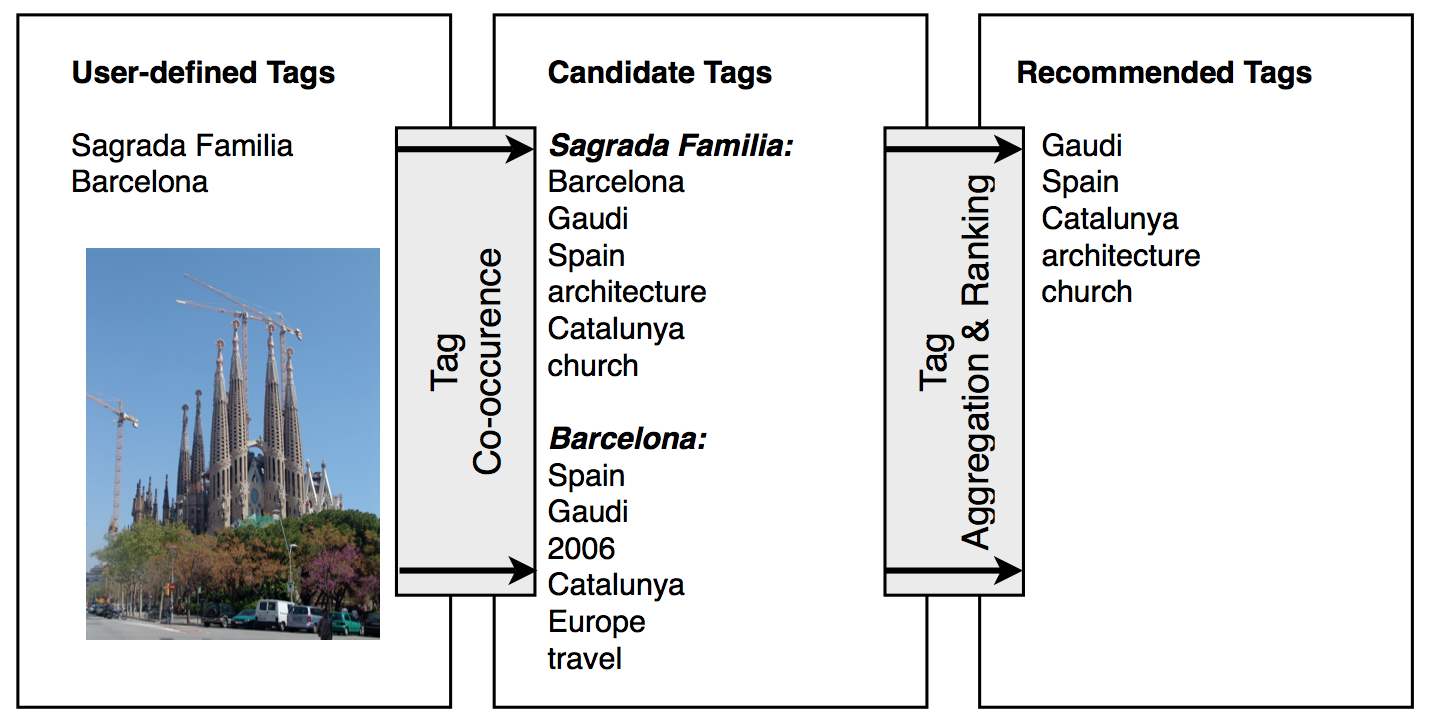
\includegraphics[height=3in]{images/collective_knowledge_system_overview.png}
  \caption{System overview of the tag recommendation process aus \cite{collectiveKnowledge}}
  \label{fig:images_collective_knowledge_system_overview}
\end{figure}


Ausführliche Beschreibung des Verfahrens folgt.

% subsection ranking_basierend_auf_kollektivem_wissen_nach_zwol_et_al_ (end)

\subsection{Verbesserung der Relevanz von Tags durch einen Random Walk nach Liu u. a.} % (fold)
\label{sub:verbesserung_der_relevanz_durch_einen_random_walk}

\begin{itemize}
  \item Wahrscheinlichkeitsorientierte Schätzung der Relevanz von Tags.
  \item Random-Walk basierte Verfeinerung des Rankings
    
    \begin{itemize}
      \item Aufbau eines Beziehungs-Graphen der Tags.
      \item Random Walk über den Graphen
    \end{itemize}
\end{itemize}

\begin{figure}[htbp]
  \centering
    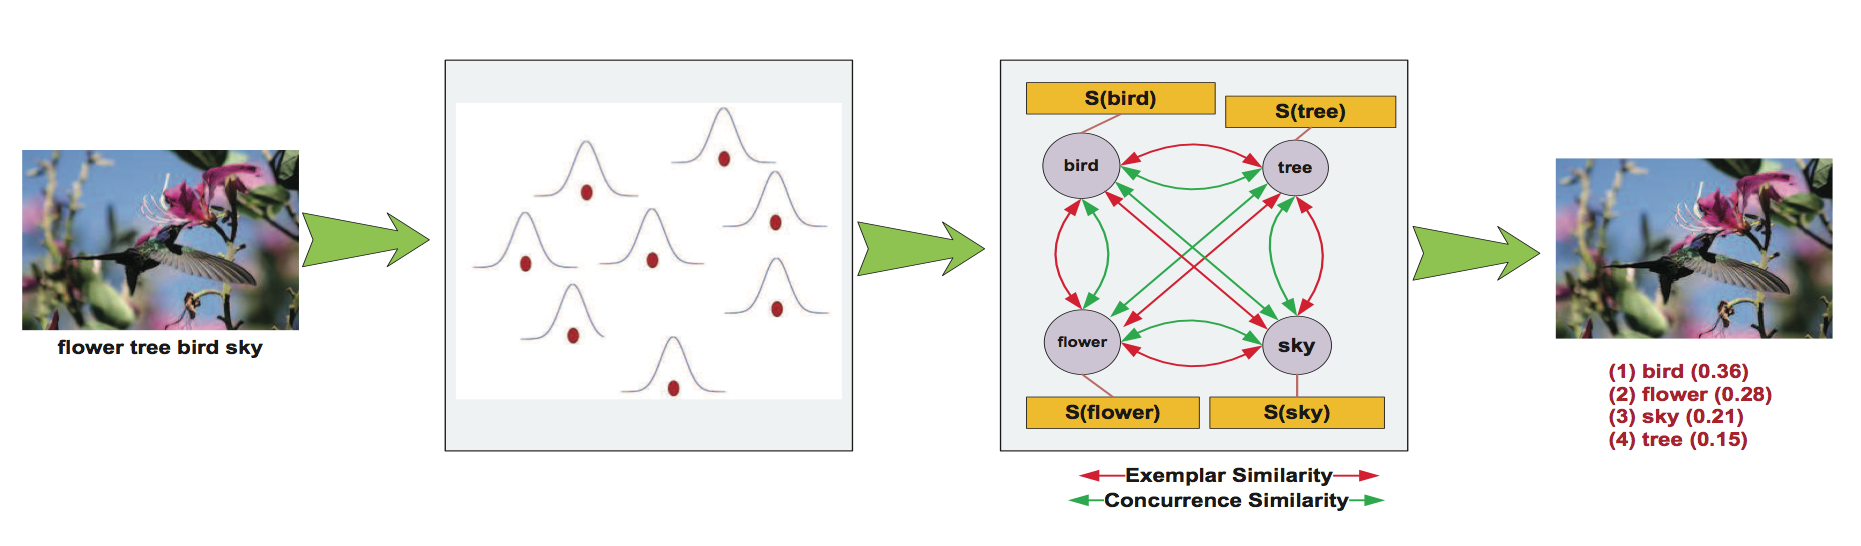
\includegraphics[height=2in]{images/tag_ranking_verfahren.png}
  \caption{The illustrative scheme of the tag ranking approach. A probabilistic method is first adopted to estimate tag relevance score. Then a random walk-based refinement is performed along the tag graph to further boost tag ranking performance aus \cite{ranking}}
  \label{fig:images_tag_ranking_verfahren}
\end{figure}


Ausführliche Beschreibung des Verfahrens folgt.

% subsection verbesserung_der_relevanz_durch_einen_random_walk (end)
% section tag_ranking_verfahren (end)

%!TEX root = /Users/ede/Documents/Master/19_AS/Ausarbeitung/as-ausarbeitung.tex
\section{Evaluation der vorgestellten Verfahren} % (fold)
\label{sec:evaluation_der_verfahren}

In diesem Kapitel erfolgt die Darstellung der Ergebnisse der jeweils von den Autoren vorgenommenen Evaluation der eingesetzten Verfahren. Dabei sollen unterschiedliche Perspektiven beleuchtet werden. Der Aufbau des Evaluationsszenarios bestimmt die Ergebnisse. Insofern soll beschrieben werden, welche Auswahl an Photos und Tags für die Evaluation verwendet wurden und ob diese nach speziellen Kriterien ausgesucht wurden. Die Art und Weise der Evaluation ist ebenfalls von Bedeutung, wobei hier zwischen automatischer und manueller bzw. durch Menschen durchgeführte Messungen der Verfahren unterschieden wird. Die Auswahl der Referenzdaten entscheidet zu welcher Basis die Verbesserungen gemessen werden und die Auswahl der Metriken entscheidet, was überhaupt gemessen wird und ob basierend darauf eine fundierte Entscheidungen über die Qualität der Verfahren getroffen werden kann. Ebenso sollte auch die Leistung und Skalierbarkeit der Algorithmen von den Autoren untersucht werden, da zum Beispiel der Einsatz solch eines Systems bei Flickr stark von der Performanz abhängt und auch für viele Milliarden von Photos und Tags funktionieren muss. Schließlich sollen die Ergebnisse der Evaluation selbst präsentiert werden.

% - aufbau des evaluationsszenarios (welche auswahl an photos und tags wurde vorgenommen,)
% - art und weise der evaluation (automatisch, manuell, was sind die referenzdaten, wie wird die qualität bewertet), welche metriken werden angewandt
% - performance der algorithmen(gibts es laufzeit analysen der algorithmen, lässt sich das verfahren skalieren)
% - qualität der ergebnisse (sind verbesserung durch das Ranking entstanden, welche methode/kombination von methoden weist das beste ranking)
% - vergleichbarkeit der ergebnisse(in wie weit ist die evaluation standardisiert, welchen mehrwert/errungenschaften hat die arbeit hervorgebracht)

\subsection{Ergebnisse der Evaluation von Sigurbjörnsson und van Zwol} % (fold)
\label{sub:ergebnisse_der_evaluation_von_collectiveknowledge}

Die Autoren von \cite{collectiveKnowledge}, Sigurbjörnsson und van Zwol, untersuchen die in Kapitel \ref{sub:ranking_basierend_auf_kollektivem_wissen_nach_zwol} vorgestellten Methoden auf ihre Leistung hin, möglichst relevante Tags zu den bereits vergebenen, benutzerdefinierten Tags vorzuschlagen. Dabei werden die eingesetzten Strategien einzeln betrachtet und evaluiert. Tabelle \ref{tab:fourStrategiesBjoern} veranschaulicht die vier untersuchten Kombinationen.

\begin{table}[htbp]
  \centering
  \begin{tabular}{c|cc}
    \hline
     & \textbf{vote} & \textbf{sum}\\
    \hline
    \textbf{no-promotion} & vote & sum\\
    \hline
    \textbf{promotion} & vote\textsuperscript{+} & sum\textsuperscript{+}\\
    \hline
  \end{tabular}
  \caption{Die vier Kombinationen von Aggregations- und Promotionsalgorithmen nach \cite{collectiveKnowledge}}
  \label{tab:fourStrategiesBjoern}
\end{table}


Die Autoren bewerten, wie das System auf unterschiedliche Anzahl bereits vorhandener Tags reagiert. Weiterhin wird untersucht, ob das Verfahren für die WordNet Kategorien aus Abbildung \ref{fig:collectiveKnowledge_word_net_categories}, Kapitel \ref{ssub:tags} unterschiedliche gute Ergebnisse liefert. Das Hauptziel ist jedoch, dass die vorgeschlagenen Tags möglichst nach ihrer Relevanz zu dem Photo sortiert sind und irrelevante Tags nicht in dieser Liste vorkommen.

\subsubsection{Aufbau des Evaluationsszenarios} % (fold)
\label{ssub:aufbau_des_evaluationsszenarios}

Die an das Tag Ranking System gestellte Aufgabe bestand also darin, zu einem Photo mit bereits vorhandenen benutzerdefinierten Tags weitere, relevante Tags vorzuschlagen. Zu diesem Zweck wurden 331 Photos zufällig aus dem Bestand von Flickr gewählt, die jedoch aus mehrere begrenzten Sachgebieten stammten, in denen die Probanden, die die Relevanz der vorgeschlagenen Tags bewerteten, sich auskennen.
Weiterhin stellten die Autoren sicher, dass die Photos möglichst gleichmäßig auf die in Kapitel \ref{sub:klassifikation_von_tags} vorgestellten Klassen aus Tabelle \ref{tab:classes_for_tags_collective} verteilt sind. Dadurch sollte überprüft werden, ob das Verfahren sich je nach Anzahl der bereits vergebenen Tags unterschiedlich verhält bzw. unterschiedlich gute Ergebnisse liefert.
  
131 dieser Photos wurden für das manuelle Training der im Algorithmus benötigten Parameter $m,	k_r,	k_s, k_d $ verwendet. Die Werte sind in Tabelle \ref{tab:optimalParameterBjoern} aufgeführt. Die restlichen 200 Photos dienten als Grundlage für die Evaluation. Dabei sollten die Probanden jedes Photo und die vom System vorgeschlagenen Tags betrachten und für die ersten 10 Tags jeweils die Beschreibbarkeit bzw. Relevanz des Tags für das Photo auf einer Skala von eins bis vier (\emph{sehr gut, gut, nicht gut, weiß nicht}) bewerten. Gleichzeitig wurden den Probanden weitere Kontextinformationen zum Photo wie Titel, Beschreibung, Aufnahmedatum usw. präsentiert, so dass diese eine möglichst fundierte Bewertung abgeben können. Die Option \emph{weiß nicht} bestand für den Fall, dass doch nicht genug Wissen für eine begründete Bewertung vorhanden war. In der Auswertung wurden die Wahlmöglichkeiten \emph{sehr gut} und \emph{gut} zu einem Wert zusammen gefasst, um eine einfachere Auswertung im Sinne von \emph{relevant} und \emph{nicht relevant} durchführen zu können.
  
\begin{table}[htbp]
  \centering
  \begin{tabular}{ccccc}
    \hline
     & \textbf{m} & \textbf{k\textsubscript{s}} & \textbf{k\textsubscript{d}} & \textbf{k\textsubscript{r}}\\
    \hline                          
    \textbf{sum} & 10 & - & - & -\\
    \hline                          
    \textbf{vote} & 10 & - & - & -\\
    \hline                          
    \textbf{sum\textsuperscript{+}} & 25 & 0 & 12 & 3\\
    \hline                          
    \textbf{vote\textsuperscript{+}} & 25 & 9 & 11 & 4\\
    \hline
  \end{tabular}
  \caption{Die optimalen Parameterwerte für $m,	k_r,	k_s, k_d$ aus \cite{collectiveKnowledge}.}
  \label{tab:optimalParameterBjoern}
\end{table}


% subsubsection aufbau_des_evaluationsszenarios (end)

\subsubsection{Metriken} % (fold)
\label{ssub:metriken}
Sigurbjörnsson und van Zwol stellen in \cite{collectiveKnowledge} drei unterschiedlich ausgerichtete Metriken zum Bewerten des Verfahrens auf. Diese sind vor allem auf die qualitativen Aspekte von Tag Ranking ausgerichtet und werden manuell, sprich durch Probandenbefragung ermittelt.
\begin{itemize}
  \item \textbf{Mean Reciprocal Rank (MRR)} misst die Position des ersten relevanten Tags in der Vorschlagsliste, gemittelt über alle bewerteten Photos. Dieser Wert sagt aus, wie gut das System in der Lage ist, die relevantesten Tags an vorderster Stelle zu positionieren.
  \item \textbf{Success at rank k (S@k)} protokolliert die Wahrscheinlichkeit, innerhalb der ersten $k$ Elemente der Vorschlagsliste relevante Tags vom System zu erhalten. Dieser Wert wird für $k = 1$ und $k = 5$ ermittelt.
  \item \textbf{Precision at rank k (P@k)} erfasst die Relation bzw. Anteil von relevanten zu irrelevanten vorgeschlagenen Tags. Dieser Wert wird ebenfalls über alle Photos gemittelt und erfasst die ersten 5 vorgeschlagenen Tags.
\end{itemize}

Als Referenzdaten wird angenommen, dass gar kein Ranking von Tags statt finden, womit klar ist, dass die Algorithmen eine grundsätzliche Verbesserung darstellen.

% subsubsection metriken (end)

\subsubsection{Ergebnisse der Evaluation} % (fold)
\label{ssub:ergebnisse_der_evaluation}

Die Ergebnisse sind in die vier Bereiche Aggregationsstrategien, Promotion, Photo Klassen und Semantisch Analyse aufgeteilt und werden im Folgenden gesondert beschrieben. Die Tabelle \ref{tab:strategiesrResultsBjoern} enthält die Ergebnisse der von \cite{collectiveKnowledge} durchgeführten Evaluation. 

\begin{table}[htbp]
  \centering
  \begin{tabular}{ccccc}
  \hline
   & \textbf{MRR} & \textbf{S@1} & \textbf{S@5} & \textbf{P@5}\\
  \hline
  Basisstrategien\\
  \textbf{sum} & .7628 & .6550 & .9200 & .4930\\
  \textbf{vote} & .6755 & .4550 & .8750 & .4730\\
  \hline
  Promototionsstrategien\\
  \textbf{sum\textsuperscript{+}} & .7718 & .6600 & .9450 & .5080\\
  \textbf{vote\textsuperscript{+}} & .7883 & .6750 & .9400 & .5420\\
  \hline
  Verbesserung durch Promotion\\
  \textbf{vote\textsuperscript{+} vs. sum} & 4.3\% & 3.1\% & 2.2\% & 9.9\%\\
  \hline
  \end{tabular}
  \caption{Die Ergebnisse der Evaluation aus \cite{collectiveKnowledge} für die Aggregation und Promotion. Die Werte geben in Prozenten die erfolgreichen, d.h. für gut oder sehr gut befundenen Ergebnisse an.}
  \label{tab:strategiesrResultsBjoern}
\end{table}

Bei der Betrachtung der zwei unterschiedlichen Aggregationsstrategien fällt auf, dass die \emph{summing strategy} bessere Ergebnisse liefert und dabei 65 Prozent aller Tags auf Position eins relevant sind. Innerhalb der ersten fünf vorgeschlagenen Tags sind in 92 Prozent der Fälle relevante Tags enthalten, wobei die Präzision bzw. der P@5 Wert aussagt, dass knapp die Hälfte der fünf ersten vorgeschlagenen Tags nicht relevant sind. Damit ist belegt, dass durch die summing Strategie der Annotationsprozess für den Benutzer verbessert werde konnte, da nun relevante Tags vorgeschlagenen werden. Gleichzeitig spricht dies für die Verwendung von co-occurence bei Tag Ranking Verfahren, da dies in der summing Strategie eingesetzt wird.

Die Einsatz der Promotion von Tags, also das Abwerten sehr hochfrequenter und sehr niederfrequenter Tags, liefert im Vergleich zu den Basisstrategien für alle Metriken bessere Ergebnisse, wobei die voting Strategie etwas bessere Resultate liefert. Die summing Strategie erzielt in Kombination mit der Promotion von Tags leicht bessere Werte in der S@5 Metrik, die voting Strategie erzielt jedoch eine bessere Präzision, das heißt es sind mehr relevante Tags in der Vorschlagsliste enthalten. Insgesamt ist den Ergebnissen nach die voting Strategie in Kombination mit der Promotion die beste Variante. Die Promotion der Tags steigert die Leistung des Verfahrens signifikant, wie in der letzten Zeile der Tabelle \ref{tab:strategiesrResultsBjoern} zu entnehmen ist.
 
Bei der Betrachtung der Photo Klassen, die nach der Anzahl ihrer benutzerdefinierten Tags unterteilt sind (siehe Tabelle \ref{tab:classes_for_tags_collective}), und der Leistung des vorgestellten Verfahrens, zeigt sich, dass die besten Ergebnisse in der Klasse I und II erreicht werden. Auch hierbei fällt auf, dass die Promotion deutlich bessere Werte für die Metriken liefert, wobei diese bei mehr benutzerdefinierten Tags stärker ausfällt als bei nur geringer Anzahl vorgegebener Tags zu einem Photo. Die Auswertung für die Photo Klassen ist in dieser Ausarbeitung nicht enthalten und kann in \cite{collectiveKnowledge}, Tabelle 5 eingesehen werden.
%TODO: Tabelle 5 könnte noch rein, dann aber auch obigen letzten satz wieder entfernen

\begin{table}[htbp]
  \centering
  \begin{tabular}{lr}
  \hline
  \textbf{WordNet} & \textbf{Akzeptanzverhältnis}\\
  \hline
  Orte & 71\%\\
  \hline
  Artefakte oder Objekte & 61\%\\
  \hline
  Andere & 53\%\\
  \hline
  Handlungen oder Ereignisse & 51\%\\
  \hline
  Zeit & 46\%\\
  \hline
  Nicht klassifiziert & 39\%\\
  \hline
  Personen oder Gruppen & 33\%\\
  \hline
  \end{tabular}
  \caption{Der Bezug zwischen WordNet Kategorien und deren Akzeptanzverhältnis durch die Probanden aus \cite{collectiveKnowledge}.}
  \label{tab:wordNetResults}
\end{table}

Die semantische Analyse fokussiert auf die in Kapitel \ref{ssub:tags}, Abbildung \ref{fig:collectiveKnowledge_word_net_categories} ermittelten WordNet Kategorien für die Tags und erfasst, welche Kategorien von Tags eine bessere Akzeptanz bzw. Relevanzwerte durch die Probanden erfahren. So soll ermittelt werden, in welchen Kategorien von Begriffen das Verfahren bessere Ergebnisse liefert. Tabelle \ref{tab:wordNetResults} zeigt das Verhältnis von gut und sehr gut befundenen Tags zu den WordNet Kategorien. Ortsbezogene Tags wurden von den Probanden am meisten akzeptiert, gefolgt von Artefakten oder Objekten und Anderen. Personen, Gruppen und nicht klassifizierte Tags, die vom System vorgeschlagen werden, erreichen nur relativ schlechte Akzeptanzwerte. Damit eignet sich das Verfahren vornehmlich für die zuerst genannten Kategorien von Begriffen.

% subsubsection ergebnisse_der_evaluation (end)

\subsubsection*{Zusammenfassung} % (fold)
\label{ssub:zusammenfassung}
Die Ergebnisse der Evaluation sprechen eindeutig für den Einsatz von co-occurence basierten Verfahren für das Ranking von Tags. Die Auswertung hat ebenso gezeigt, dass auch die Analyse der bereits vorhanden Tags und das Einfließen dieser Analyse in Form von Promotion im Verfahren in einer verbesserten Leistung des Algorithmus resultiert.

Die Evaluation von Sigurbjörnsson und van Zwol bezieht sich jedoch nur auf die qualitativen Aspekten des Ranking Verfahrens. Quantitative Messungen zu Skalierbarkeit und Laufzeit wurden nicht durchgeführt. 
% subsubsection zusammenfassung (end)

% subsection ergebnisse_der_evaluation_von_collectiveknowledge (end)

\subsection{Ergebnisse der Evaluation von Liu u. a.} % (fold)
\label{sub:ergebnisse_der_evaluation_von_liu}

Ziel der Evaluation von Liu u. a. war die Erfolgsquote der beiden Hauptmethoden des Verfahrens, Initiale stochastische Schätzung des Tag Ranking Wertes und die Verbesserung des Tag Rankings durch einen Random Walk, im Einzelnen und in Kombination. Dazu wurden die Tags durch Probanden nach ihrer Relevanz zum zugehörigen Photo bewertet und anschließend mit Hilfe der NDCG Messung, die in Abschnitt \ref{ssub:metriken_liu} näher erläutert wird, evaluiert.

\subsubsection{Aufbau des Evaluationsszenarios} % (fold)
\label{ssub:aufbau_des_evaluationsszenarios_liu}
Um die Testdaten für die Evaluation zu sammeln, wurde zunächst eine Auswahl von zehn populären Tags aus Flickr getroffen. Für jeden Tag wurde eine Suche bei Flickr mit Begrenzung auf die ersten 5000 Photo durchgeführt, so dass eine Sammlung von 50.000 Testphotos inklusive der anhängenden Informationen wie Tags, Aufnahmezeit usw. aufgebaut wurde.

Auch in \cite{ranking} wurden die Testphotos und deren Tags einer Vorfilterung unterzogen. Dabei wurden Tags entfernt, die nicht im Thesaurus von Wikipedia enthalten waren. Dies ist damit begründet, dass viele Tags falsch geschriebene oder bedeutungslose Begriffe sind. Dadurch wurde die Menge von anfänglich mehr als 100.000 Tags auf 13.330 reduziert.

Aus der Gesamtmenge der Testphotos wurden daraufhin 10.000 Photos für die Evaluation eingesetzt. Fünf Probanden bewerteten die Tags aller Photos auf einer Skala von eins bis fünf, wobei folgende Wertungen abgegeben werden konnten: \emph{sehr relevant(5)}, \emph{relevant(4)}, \emph{teilweise relevant(3)}, \emph{schwach relevant(2)} und \emph{nicht relevant(1)}.
% subsubsection aufbau_des_evaluationsszenarios_liu (end)

\subsubsection{Metriken} % (fold)
\label{ssub:metriken_liu}

In \cite{ranking} wird zur Bewertung der Ergebnisse und vor allem deren Reihenfolge die \emph{Discounted cumulative gain}(DCG) Methode nach \cite{ndcg} verwendet. Diese Messmethode erfasst die Effektivität von Suchalgorithmen und verwandten Verfahren, wobei die Nützlichkeit (englisch: \emph{gain}) der einzelnen Elemente anhand ihrer Position in dem Suchergebnis und der Relevanz des Elementes gemessen wird. Als Vergleichsbasis der Messung dient eine Relevanzskala wie sie in Abschnitt \ref{ssub:aufbau_des_evaluationsszenarios_liu} beschrieben wurde. Der NDCG ist der \emph{normalized} DCG, welcher die Ergebnisse einer Messung auf einen Wert zwischen 0 und 1 normalisiert, so dass mehrere Suchanfrage miteinander verglichen werden können. Gleichung \ref{fig:ndcg} führt die Funktion zur Berechnung des NDCG für eine mit dem Verfahren gewertete Tag Liste $t_1, t_2, ..., t_n$ auf. $r(i)$ ist hierbei der Relevanzwert vom $i$-ten Tag und $Z_n$ ist die eben beschriebene Normalisierungskonstante.
\begin{figure}[hptb]
  \begin{equation}
  \label{fig:ndcg}
    N_n = Z_n \sum_{i=1}^n(2^{r(i)} - 1) / log(1+i)
  \end{equation}
\end{figure}

Nachdem für jede, gerankte Tag Liste eines Photos der NDCG ermittelt wurde, können die Werte gemittelt werden, so dass allgemeine Aussagen über alle Tags und Photos hinweg getroffen werden können. Je näher der NDCG Wert bei 1 liegt, desto relevanter sind die Ergebnisse in Bezug zum Suchwort. Im vorliegenden Fall wäre dies die Relevanz der Tags zum gezeigten Photo.
% subsubsection metriken_liu (end)

\subsubsection{Ergebnisse der Evaluation} % (fold)
\label{ssub:ergebnisse_der_evaluation_liu}

Obwohl Liu u. a. die Kombination von stochastischer Schätzung und Random Walk für das Berechnen von Tag Ranking Werte vorschlagen, haben Sie die beiden Methoden einzeln und in Kombination untersucht. Die Referenzwerte für die Evaluation wurden hierbei aus der originalen, von Flickr gelieferten Tag Liste bezogen. Die Ergebnisse der Messung der Verfahren mittels NDCG ist an Abbildung \ref{fig:images_ndcgAll} dargestellt.
\begin{figure}[htbp]
  \centering
    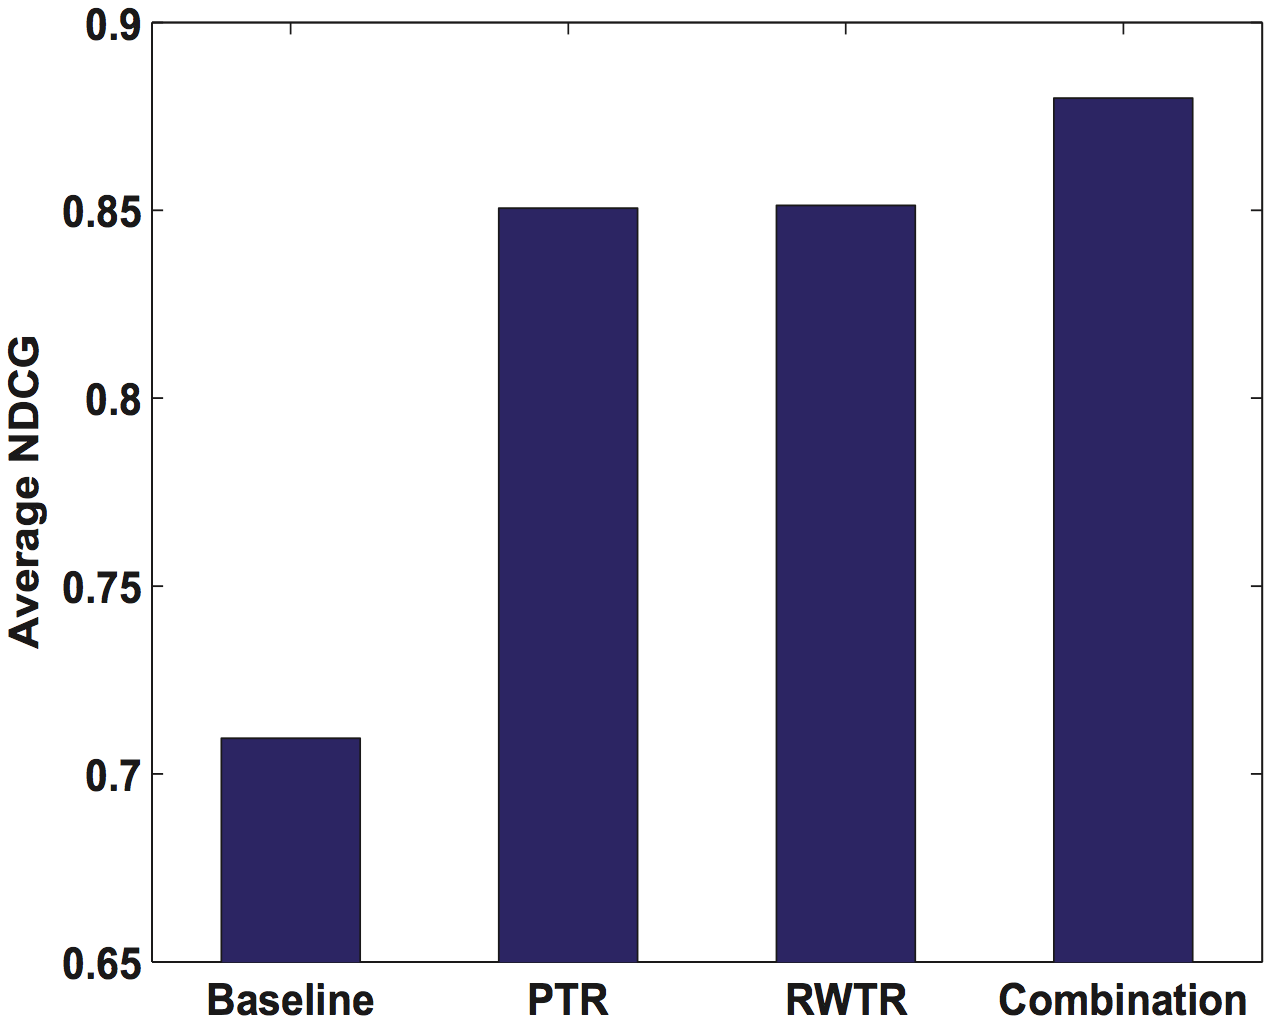
\includegraphics[height=3in]{images/ndcgAll.png}
  \caption{Messergebnisse der unterschiedlichen Tag Ranking Methoden. \emph{Baseline} ist der Wert für die Flickr Tag Liste. \emph{PTR} bezeichnet die stochastische Schätzung, \emph{RWTR} die Random Walk Ranking Methode. \emph{Combination} ist die Kombination beider Methoden.}
  \label{fig:images_ndcgAll}
\end{figure}

An der Grafik erkennt man gut, dass bereits die Tag Liste von Flickr die Tags nach ihrer Relevanz sortiert enthält, die vorgestellten Methoden nach \cite{ranking} jedoch signifikante Verbesserung mit sich bringen. Dabei ist die Kombination von stochastischer Schätzung und dem Random Walk die beste Alternative. Hierbei wird ein NDCG Wert von ca. 0,88 erreicht, was einer sehr hohen Relevanz der Tags zum Photo entspricht.

Vergleicht man die Position des relevantesten Tags vor dem Tag Ranking in Abbildung \ref{fig:images_tag_ranking_psotion_relevant_tag} und nach der Anwendung des Verfahrens in Abbildung \ref{fig:images_positionRelevantTags}, so erkennt man, dass nun ca. 40 Prozent aller Photos ihren relevantesten Tag an erster Position haben, was eine Verbesserung um knapp 30 Prozent darstellt. Das Verfahren erzielt somit eine gute Leistung bei der Ermittlung der relevantesten Tags zu einem Photo.

\begin{figure}[htbp]
  \centering
    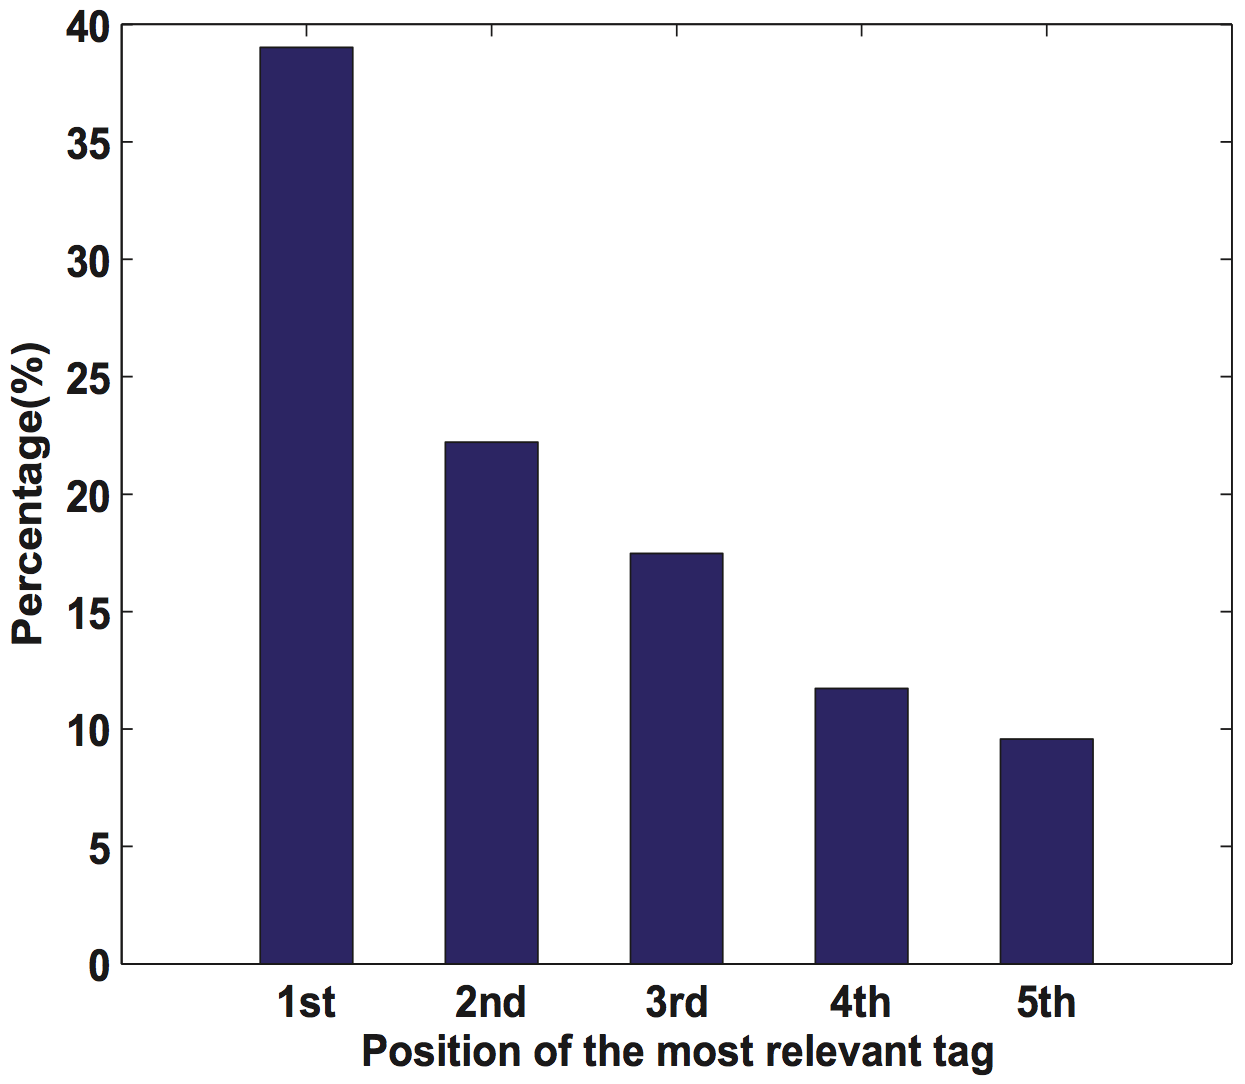
\includegraphics[height=3in]{images/positionRelevantTags.png}
  \caption{Prozentuale Anteile der Tags nach dem Ranking, die ihren relevantesten Tag an n-ter Position haben, aus \cite{ranking}.}
  \label{fig:images_positionRelevantTags}
\end{figure}


% subsubsection ergebnisse_der_evaluation_liu (end)

\subsubsection*{Zusammenfassung} % (fold)
\label{ssub:zusammenfassung_und_bewertung_liu}
Liu u. a. belegen durch die durchgeführte Evaluation eine eindeutige Verbesserung der Relevanz von Tags durch Anwendung ihres Ranking Verfahrens. Vor allem konnte eine bessere Leistung bei der Priorisierung des ersten Tags nachgewiesen werden. 

Eine Analyse der Laufzeit des Algorithmus fehlt ebenso wie Untersuchungen zur Skalierbarkeit. 


% subsubsection zusammenfassung_und_bewertung_liu (end)
% subsection ergebnisse_der_evaluation_von_ (end)

% section performance_und_skalierung (end)

%!TEX root = /Users/ede/Documents/Master/19_AS/Ausarbeitung/as-ausarbeitung.tex
\section{Vergleich und Bewertung der Verfahren} % (fold)
\label{sec:vergleich_und_bewertung_der_verfahren}
Gegenüberstellung der Verfahren, mit aufzeigen der Parallelen, der Unterschiede, jeweiligen Vor- und Nachteile und anschließender Bewertung.


- van zwol: 
 - manuelle evaluation
 - fraglich, warum nicht beide verfahren(summing + voting) in kombination eingesetzt wurden
 - evaluation deutlich auf die Anwendung des Tag Rankings für das Vorschlagen ausgerichtet.
 
- liu:
 - es werden nur bereits vergebene Tags in der Evaluation betrachtet und somit kann nur deren Sortierung nach Relevanz verbessert werden.

% section vergleich_und_bewertung_der_verfahren (end)

%!TEX root = /Users/ede/Documents/Master/19_AS/Ausarbeitung/as-ausarbeitung.tex
\section{Fazit}
In dieser Arbeit wurde vorgestellt, warum die manuelle Annotation von Multimedia, das Tagging, zur Zeit noch die sinnvollere Variante der Metadatenerstellung ist und welche Potentiale daraus für die Suche nach Multimedia entstehen. Die Analyse von Tags der Folksonomy von Flickr offenbart mehrere Probleme die durch das Tagging entstehen, welche jedoch durch die Tag Ranking Verfahren reduziert werden sollen. Gleichzeitig verspricht die Anwendung dieser Verfahren eine bessere Sortierung der Ergebnisse einer Suche nach ihrer Relevanz und einen einfacheren Annotationsprozess für den Benutzer. %Die momentan in Flickr vorhandenen Tags enthalten keine Relevanzwerte

Es werden also vielfältige Anforderungen an ein Tag Ranking Verfahren gestellt, so dass von den Autoren zunächst eine Analyse der bereits vorhanden Tags durchgeführt wurde. Die Analyse beantwortet Fragen über die Häufigkeitsverteilung von Tags, die Beziehungen der Tags über die Photos, welche Art von Inhalten die Benutzer annotieren und weiter statistische Daten. Basierend darauf erfolgt eine Klassifikation der Photos und Tags, welche in der späteren Evaluation Verwendung findet.

Der Ansatz von Sigurbjörnsson und van Zwol fokussiert auf den Wert der co-occurrence von zwei Tags. Basierend darauf wurden zwei Aggregationsstrategien vorgestellt, um die Kandidatensequenzen für benutzerdefinierte Tags zu ermitteln und zu einer, nach der Relevanz sortierten Sequenz, zusammen zu führen. Daraufhin erfolgt die Einbeziehung der Analyse, wobei extrem hoch- und niederfrequente Tags abgewertet werden. Das Verfahren eignet sich damit zum Vorschlagen von Tags bei der Annotation von Photos durch den Benutzer.

Die Autoren von \cite{ranking} gehen einen anderen Weg und schätzen zunächst mit Hilfe einer stochastischen Methodik einen initialen Ranking Wert für jeden Tag eines Photos. Daraufhin wird ein Tag Graph konstruiert, wobei die Ähnlichkeit von Photos mit einbezogen wird und ein Random Walk ausgeführt wird. Die Methode des Random Walk ist in dem Gebiet des Information Retrieval etabliert und resultiert in guten Ergebnissen bei der Ermittlung von Relevanzwerten durch die Beziehung der einzelnen Tags untereinander.

Beide Arbeiten werden durch eine ausführliche Evaluation der Ranking Verfahren abgeschlossen. Hierin weisen Sie nach, dass die Verwendung der vorgestellten Ranking Verfahren deutliche Verbesserungen in den Anwendungsgebieten von Tags, wie dem Vorschlagen von Tags bei der Annotation oder der tagbasierten Suche nach Multimedia Objekten, zur Folge hat.

\bibliography{bib/literatur}

% \bibliographystyle{dinat}
% \bibliographystyle{plaindin}
\bibliographystyle{alpha}


\end{document}
